\documentclass[11pt,a4paper]{article}

%==============================================================================
%  DMRG++: A pedagogical companion to the source code
%
%  This document is intentionally self-contained.  Compile with:
%      latexmk -pdf dmrg_pedagogical.tex
%  or
%      pdflatex dmrg_pedagogical.tex && pdflatex dmrg_pedagogical.tex
%==============================================================================

\usepackage[utf8]{inputenc}
\usepackage[T1]{fontenc}
\usepackage{lmodern}
\usepackage{microtype}
\usepackage[margin=1in]{geometry}

\usepackage{amsmath,amssymb,amsthm,mathtools}
\usepackage{bm}
\usepackage{braket}
\usepackage{physics}
\usepackage{graphicx}
\usepackage{tikz}
\usetikzlibrary{calc,positioning,shapes.geometric,arrows.meta,decorations.pathreplacing}
\usepackage{xcolor}
\usepackage{listings}
\usepackage{enumitem}
\usepackage{booktabs}
\usepackage{caption}
\usepackage[hidelinks,colorlinks=true,linkcolor=blue!50!black,citecolor=blue!50!black,urlcolor=teal!60!black]{hyperref}
\usepackage{cleveref}

%------------------------------------------------------------------ theorem env
\theoremstyle{plain}
\newtheorem{theorem}{Theorem}[section]
\newtheorem{lemma}[theorem]{Lemma}
\newtheorem{proposition}[theorem]{Proposition}
\theoremstyle{definition}
\newtheorem{definition}[theorem]{Definition}
\newtheorem{example}[theorem]{Example}
\theoremstyle{remark}
\newtheorem*{remark}{Remark}

%------------------------------------------------------------------ code style
\definecolor{codebg}{RGB}{248,248,248}
\definecolor{codekw}{RGB}{0,0,180}
\definecolor{codestr}{RGB}{0,128,0}
\definecolor{codecom}{RGB}{120,120,120}
\lstdefinelanguage{pythonlike}{
  morekeywords={def,class,return,for,while,if,elif,else,import,from,as,with,
                in,not,and,or,True,False,None,lambda,yield,raise,try,except,
                finally,pass,break,continue,global,nonlocal,assert,self},
  sensitive=true,
  morecomment=[l]{\#},
  morestring=[b]",
  morestring=[b]'
}
\lstset{
  language=pythonlike,
  basicstyle=\ttfamily\small,
  backgroundcolor=\color{codebg},
  keywordstyle=\color{codekw}\bfseries,
  stringstyle=\color{codestr},
  commentstyle=\color{codecom}\itshape,
  showstringspaces=false,
  frame=single,
  framerule=0pt,
  xleftmargin=12pt,
  xrightmargin=4pt,
  breaklines=true,
  columns=fullflexible,
}

%------------------------------------------------------------------ shortcuts
\newcommand{\Id}{\mathbb{1}}
\newcommand{\R}{\mathbb{R}}
\newcommand{\C}{\mathbb{C}}
\newcommand{\Z}{\mathbb{Z}}
\newcommand{\Hilb}{\mathcal{H}}
\renewcommand{\op}[1]{\hat{#1}}
\newcommand{\eps}{\varepsilon}
\newcommand{\dphys}{d}
\newcommand{\Dvirt}{D}
\newcommand{\Dmpo}{D_{\!w}}
% Pretty-print a path to a file relative to the repo root.  We use \path
% from the url package (loaded via hyperref) so that long file paths break
% naturally at directory separators and underscores render verbatim.
\newcommand{\codefile}[1]{\path{#1}}

%------------------------------------------------------------------ tikz styles
\tikzset{
  tensor/.style={
    draw,
    minimum size=8mm,
    inner sep=0pt,
    line width=0.5pt,
    fill=blue!8,
  },
  mpotensor/.style={
    draw,
    rectangle,
    minimum width=8mm,
    minimum height=8mm,
    fill=orange!12,
    line width=0.5pt,
  },
  envtensor/.style={
    draw,
    rectangle,
    minimum width=10mm,
    minimum height=14mm,
    fill=green!10,
    line width=0.5pt,
  },
  bond/.style={line width=0.6pt},
  phys/.style={line width=0.6pt, dashed},
}

%------------------------------------------------------------------ title
\title{\bfseries DMRG\textsuperscript{++}: A Pedagogical Companion\\
{\large Density Matrix Renormalization Group, from first principles to working code}}
\author{Documentation for the \texttt{dmrg\_pp} library}
\date{\today}

\begin{document}
\maketitle
\begin{abstract}
\noindent
This document is the theoretical and algorithmic companion to the
\texttt{dmrg\_pp} library.  It develops everything needed to understand the
two-site finite-system Density Matrix Renormalization Group (DMRG) algorithm
from scratch --- starting with the curse of dimensionality of quantum many-body
problems and ending with a fully derived effective-Hamiltonian update --- and
maps every concept to a concrete location in the source tree.  The intended
audience is a graduate student or researcher who has seen quantum mechanics and
linear algebra but has never worked with tensor networks before.
\end{abstract}

\tableofcontents
\bigskip\hrule\bigskip


%==============================================================================
\section{Why DMRG?}
\label{sec:why}

A quantum lattice model on $L$ sites with local Hilbert space dimension
$\dphys$ lives in
\begin{equation}
  \Hilb_L = \bigotimes_{i=0}^{L-1} \C^{\dphys}, \qquad
  \dim \Hilb_L = \dphys^{L}.
\end{equation}
For a spin-$\tfrac12$ chain ($\dphys=2$) on $L=50$ sites this is already
$\approx 1.13\times 10^{15}$ complex amplitudes --- larger than the memory of
any conceivable single computer.  Exact diagonalization is therefore limited
to $L \lesssim 30$ in practice.

DMRG escapes this barrier by exploiting a remarkable empirical fact: the
ground states of \emph{gapped, local} 1D Hamiltonians have only \emph{area-law}
entanglement\footnote{Hastings (2007) made this rigorous: the ground state of
a gapped, local 1D Hamiltonian satisfies $S(\rho_A) \le c$ for some constant
$c$ independent of $|A|$.  Critical (gapless) systems satisfy a logarithmic
correction $S \sim \tfrac{c}{6}\log L$ from CFT.}.  An area-law state on a 1D
chain can be compressed into a \emph{Matrix Product State} (MPS) of bounded
bond dimension, with cost \emph{linear} in $L$.  DMRG is the variational
algorithm that finds the optimal MPS approximation to the ground state.

\medskip
\noindent\textbf{Code orientation.}
The library top level (\codefile{src/dmrg_pp/__init__.py}) re-exports the
five user-facing names that drive most calculations:
\begin{lstlisting}
from dmrg_pp import MPS, MPO, MPOBuilder, DMRGConfig, run_dmrg
\end{lstlisting}
We will derive what each of these represents and how they fit together.


%==============================================================================
\section{Tensor-network notation in 90 seconds}
\label{sec:tn}

A rank-$n$ tensor is, for our purposes, just an $n$-index numerical array
$T_{a_1 a_2 \cdots a_n}$.  We draw it as a node with $n$ legs:

\begin{center}
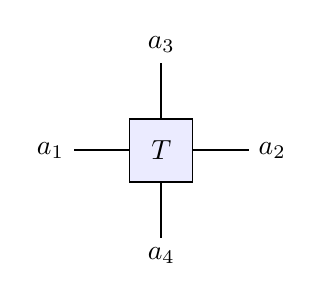
\begin{tikzpicture}[baseline=-1mm]
  \node[tensor] (T) {$T$};
  \draw[bond] (T.west)  -- ++(-0.7,0) node[left]{$a_1$};
  \draw[bond] (T.east)  -- ++(+0.7,0) node[right]{$a_2$};
  \draw[bond] (T.north) -- ++(0,+0.7) node[above]{$a_3$};
  \draw[bond] (T.south) -- ++(0,-0.7) node[below]{$a_4$};
\end{tikzpicture}
\end{center}

Connecting two legs means summing over their shared index --- i.e.\ a
contraction:
\begin{equation}
  C_{ac} = \sum_b A_{ab}\,B_{bc}
  \quad\Longleftrightarrow\quad
  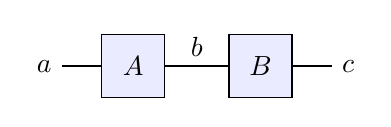
\begin{tikzpicture}[baseline=-1mm]
    \node[tensor] (A) {$A$};
    \node[tensor, right=8mm of A] (B) {$B$};
    \draw[bond] (A.east) -- node[above]{$b$} (B.west);
    \draw[bond] (A.west) -- ++(-0.5,0) node[left]{$a$};
    \draw[bond] (B.east) -- ++(+0.5,0) node[right]{$c$};
  \end{tikzpicture}.
\end{equation}
This is the entire graphical calculus.  In the code, contractions are
\texttt{numpy.tensordot} calls; the explicit axis lists in our routines are
exactly the legs being joined in the diagram.


%==============================================================================
\section{Matrix Product States}
\label{sec:mps}

\subsection{Definition}

A wave-function $\ket{\psi} \in \Hilb_L$ has $\dphys^L$ amplitudes
$\psi_{\sigma_0 \sigma_1 \cdots \sigma_{L-1}}$.  A \emph{Matrix Product State}
factorises these amplitudes as a chain of matrix products,
\begin{equation}
  \boxed{\;
  \psi_{\sigma_0 \sigma_1 \cdots \sigma_{L-1}}
  \;=\;
  \sum_{a_1,\dots,a_{L-1}}
  M^{\sigma_0}_{1,\,a_1}\,
  M^{\sigma_1}_{a_1,\,a_2}\,
  \cdots
  M^{\sigma_{L-1}}_{a_{L-1},\,1}\;}
\end{equation}
where for each site $i$ and each physical configuration $\sigma_i$,
$M^{\sigma_i}$ is a $\Dvirt_i \times \Dvirt_{i+1}$ matrix.  The
\emph{virtual} (or \emph{bond}) dimensions $\Dvirt_i$ control the amount of
entanglement the state can carry; the boundary bonds $\Dvirt_0 = \Dvirt_L = 1$
make the outer brackets reduce to scalars.

Diagrammatically:

\begin{center}
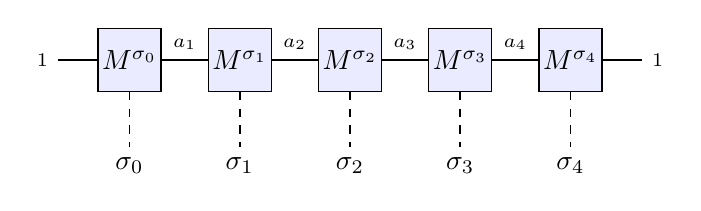
\begin{tikzpicture}[node distance=10mm and 8mm]
  \foreach \i [count=\j from 0] in {0,1,2,3,4} {
    \node[tensor] (M\j) at (\j*1.4, 0) {$M^{\sigma_{\i}}$};
    \draw[phys] (M\j.south) -- ++(0,-0.7) node[below]{$\sigma_{\i}$};
  }
  \foreach \j in {0,1,2,3} {
    \pgfmathtruncatemacro{\jp}{\j+1}
    \draw[bond] (M\j.east) -- (M\jp.west) node[midway,above]{\scriptsize $a_{\jp}$};
  }
  \draw[bond] (M0.west) -- ++(-0.5,0) node[left]{\scriptsize $1$};
  \draw[bond] (M4.east) -- ++(+0.5,0) node[right]{\scriptsize $1$};
\end{tikzpicture}
\end{center}

Each tensor $M^{\sigma_i}$ corresponds to a single rank-3 NumPy array of shape
$(\Dvirt_i,\,\dphys,\,\Dvirt_{i+1})$, with the convention:

\smallskip
\begin{center}\small
  axis 0 $=$ left virtual bond, \quad
  axis 1 $=$ physical leg, \quad
  axis 2 $=$ right virtual bond.
\end{center}
\smallskip

This is exactly the layout enforced by the constructor of
\codefile{src/dmrg_pp/states/mps.py}:
\begin{lstlisting}
def __init__(self, tensors, *, centre=None, copy=True):
    ...
    if t.ndim != 3:
        raise ValueError(f"site {i}: tensor must be rank-3, got ndim={t.ndim}")
    if t.shape[0] != prev_right:
        raise ValueError(f"site {i}: left bond {t.shape[0]} != "
                         f"previous right bond {prev_right}")
\end{lstlisting}

\subsection{Why this is a good idea}

The total parameter count of an MPS with bounded bond dimension
$\Dvirt_i \le \chi$ is
\begin{equation}
  \#\text{params} \;\le\; L\,\dphys\,\chi^2,
\end{equation}
which is \emph{linear} in $L$.  This is exponentially smaller than $\dphys^L$
the moment $\chi$ is bounded.  The non-trivial physics statement is that for
gapped local 1D Hamiltonians, $\chi$ \emph{can} be bounded (independent of
$L$, modulo polylog corrections at criticality) while still capturing the
ground-state physics to any desired accuracy.

\subsection{Canonical forms}
\label{sec:canonical}

The MPS representation is \emph{not unique}: inserting any invertible matrix
$X$ on a bond and its inverse $X^{-1}$ on the next site gives a different
representation of the same wave-function.  We exploit this gauge freedom to
put the MPS into a convenient \emph{canonical form}.

\begin{definition}[Left- and right-canonical sites]
A site tensor $A^{\sigma}_{a,b}$ is \textbf{left-canonical} if, viewed as a
$(\Dvirt\dphys) \times \Dvirt'$ matrix, it is a left-isometry:
\begin{equation}
  \sum_{a,\sigma} (A^{\sigma}_{a,b})^{*}\,A^{\sigma}_{a,b'}
  \;=\; \delta_{b\,b'}.
\end{equation}
\textbf{Right-canonical} sites satisfy the mirror condition $\sum_{\sigma,b}
A^{\sigma}_{a,b}\,(A^{\sigma}_{a',b})^{*} = \delta_{a\,a'}$.
\end{definition}

\begin{definition}[Mixed canonical form]
An MPS is in \textbf{mixed canonical form with orthogonality centre} $c$ if
sites $i<c$ are left-canonical, sites $i>c$ are right-canonical, and the
centre site carries the entire normalisation:
\begin{equation}
  \norm{\psi}^2 \;=\; \norm{M^{(c)}}_{F}^{2}.
\end{equation}
\end{definition}

Moving the centre by one site costs a single \textbf{QR decomposition} ---
this is what the helpers \texttt{\_left\_canonicalize\_site} and
\texttt{\_right\_canonicalize\_site} of the \texttt{MPS} class do in
\codefile{src/dmrg_pp/states/mps.py}.  The class tracks the current centre
in \texttt{self.\_centre} so that subsequent operations (norms, local
expectation values, \ldots) are $\mathcal{O}(1)$ rather than $\mathcal{O}(L)$.

\paragraph{Why we sign-fix the QR.}  The QR decomposition is unique only up
to a diagonal unitary; standard LAPACK does not fix this freedom.  Our
implementation in \codefile{src/dmrg_pp/tensors/linalg.py} forces the diagonal
of $R$ to be real and non-negative, so that $\texttt{left\_qr}(A)$ is a
deterministic function of $A$ --- crucial for reproducible tests.


%==============================================================================
\section{Truncated SVD: the workhorse}
\label{sec:svd}

The single most important fact in DMRG is the optimality of singular-value
truncation.

\begin{theorem}[Eckart--Young--Mirsky]
Let $M \in \C^{m\times n}$ have SVD $M = U\Sigma V^{\dagger}$ with singular
values $s_1 \ge s_2 \ge \cdots \ge s_{\min(m,n)} \ge 0$.  Then for any $\chi$,
the matrix $M_{\chi} = U_{:\chi}\Sigma_{\chi} V_{:\chi}^{\dagger}$ obtained by
keeping only the largest $\chi$ singular values is the unique\footnote{Up to
genuine spectral degeneracies in the singular values $s_\chi = s_{\chi+1}$.}
minimiser of $\norm{M - X}_F$ over all rank-$\chi$ matrices $X$.  The
truncation error is
\begin{equation}
  \norm{M - M_{\chi}}_{F}^{2} \;=\; \sum_{i>\chi} s_{i}^{2}.
\end{equation}
\end{theorem}

In MPS language, this means: if we want to compress a bond from dimension
$\Dvirt$ down to $\chi$, the SVD prescription is \emph{provably optimal}.

The DMRG sweep engine of \cref{sec:dmrg-engine} truncates after every two-site
update.  The library exposes the relevant primitive in
\codefile{src/dmrg_pp/tensors/linalg.py}:

\begin{lstlisting}
def truncated_svd(matrix, *, max_bond=None, cutoff=0.0,
                  min_bond=1, renormalize=False):
    """Truncated SVD with rich diagnostics.

    Decomposes  matrix  ~  U @ diag(s) @ Vh  keeping at most max_bond
    singular values and discarding any with cumulative weight below
    cutoff * sum(s**2).
    """
\end{lstlisting}

The \emph{relative} cutoff convention (relative to the total Frobenius weight
$\sum_i s_i^2$) is the same one used by ITensor and TenPy.  We return a
\texttt{TruncationInfo} dataclass containing the kept singular spectrum, the
discarded weight, the largest discarded value, and the resulting bond
dimension --- all of which the DMRG sweep engine logs and persists.


%==============================================================================
\section{Matrix Product Operators}
\label{sec:mpo}

An MPO factorises an operator $\op H : \Hilb_L \to \Hilb_L$ as
\begin{equation}
  \op H \;=\; \sum_{\{w\}}
    W^{\sigma_0 \tau_0}_{1,\,w_1}\,
    W^{\sigma_1 \tau_1}_{w_1,\,w_2} \cdots
    W^{\sigma_{L-1} \tau_{L-1}}_{w_{L-1},\,1}\,
    \ket{\bm\sigma}\bra{\bm\tau}.
\end{equation}
Each tensor $W$ at site $i$ is a rank-4 array of shape
$(\Dmpo,\,\dphys,\,\dphys,\,\Dmpo')$ with leg ordering
\smallskip
\begin{center}\small
  (left bond, $\sigma$ output, $\tau$ input, right bond).
\end{center}
\smallskip
Diagrammatically:

\begin{center}
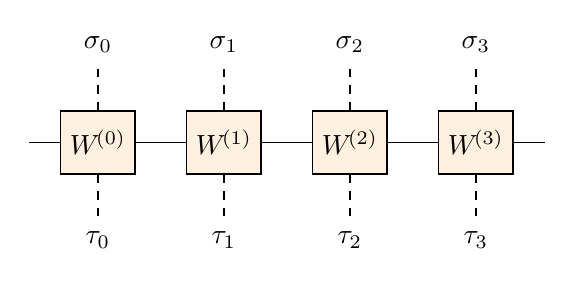
\begin{tikzpicture}[node distance=10mm and 8mm]
  \foreach \i [count=\j from 0] in {0,1,2,3} {
    \node[mpotensor] (W\j) at (\j*1.6, 0) {$W^{\!(\i)}$};
    \draw[phys] (W\j.north) -- ++(0,+0.6) node[above]{$\sigma_{\i}$};
    \draw[phys] (W\j.south) -- ++(0,-0.6) node[below]{$\tau_{\i}$};
  }
  \foreach \j in {0,1,2} {
    \pgfmathtruncatemacro{\jp}{\j+1}
    \draw[bond] (W\j.east) -- (W\jp.west);
  }
  \draw[bond] (W0.west) -- ++(-0.4,0);
  \draw[bond] (W3.east) -- ++(+0.4,0);
\end{tikzpicture}
\end{center}

The \emph{action} convention is the natural one,
$(\op H \ket{\psi})_{\bm\sigma} = \sum_{\bm\tau} H_{\bm\sigma,\bm\tau}
\psi_{\bm\tau}$, so $\sigma$ is the \emph{output} (ket) leg and $\tau$ the
\emph{input} (bra) leg.  This is enforced in
\codefile{src/dmrg_pp/operators/mpo.py}.

\subsection{The finite-state-machine MPO builder}
\label{sec:fsm}

How do we obtain the local $W$ tensors for a Hamiltonian like the Heisenberg
chain
\begin{equation}
  \op H_{\mathrm{XXZ}} \;=\;
  \sum_{i=0}^{L-2}
  \left[\,
    \tfrac{J_{xy}}{2}\bigl(\op S^{+}_i \op S^{-}_{i+1}
                          + \op S^{-}_i \op S^{+}_{i+1}\bigr)
    + J_z \op S^{z}_i \op S^{z}_{i+1}
  \,\right] \;+\; h \sum_i \op S^{z}_i\;?
\end{equation}
The cleanest construction views the MPO as a finite-state automaton on the
virtual bond.  The bond at position $b$ carries three classes of states:

\begin{enumerate}[leftmargin=2em,label=(\alph*)]
\item \textbf{Start}: ``no Hamiltonian term has begun yet to my left.''
\item \textbf{Transit$_\alpha$}: ``term $\alpha$ has begun but not yet
      finished'' --- one bond state per term currently in flight.
\item \textbf{End}: ``every term whose support is to my left has finished
      emitting.''
\end{enumerate}

The local $W$ tensors are the transition matrices of this automaton,
decorated with the local operators for the transitions that emit them.  The
``always identity'' loops on \textbf{Start} and \textbf{End} ensure that
terms whose support has not yet (or already) been visited contribute the
identity locally.

\begin{example}[Transverse-field Ising chain]
For
$\op H = -J\sum_i \sigma^z_i \sigma^z_{i+1} - g\sum_i \sigma^x_i$
the FSM has $D=3$: \{Start, Transit$_{Z}$, End\}.  The internal $W$ tensors
read, in the basis (Start, Transit$_Z$, End):
\begin{equation}
  W \;=\;
  \begin{pmatrix}
    \op{\Id}        & \sigma^z & -g\,\sigma^x \\
    0              & 0        & -J\,\sigma^z \\
    0              & 0        & \op{\Id}
  \end{pmatrix},
\end{equation}
which is exactly the well-known $D=3$ Ising MPO.\footnote{Reading entries
right-to-left: the lower-right $\op{\Id}$ block is ``stay in End''; the
upper-left $\op{\Id}$ is ``stay in Start''; the column above End reads ``end
the term by emitting $-g\sigma^x$ (single-site) or $-J\sigma^z$ (closing a
two-site term)''.}
\end{example}

\noindent
This construction is implemented in \codefile{src/dmrg_pp/operators/builder.py}.
The user-facing API is symbolic:

\begin{lstlisting}
from dmrg_pp.operators.builder import MPOBuilder
from dmrg_pp.operators.local_ops import spin_half_ops

ops = spin_half_ops()
b = MPOBuilder(L=L, local_ops=ops)
for i in range(L - 1):
    b.add(0.5,  (i, "Sp"), (i + 1, "Sm"))
    b.add(0.5,  (i, "Sm"), (i + 1, "Sp"))
    b.add(1.0,  (i, "Sz"), (i + 1, "Sz"))
mpo = b.build()                # produces D=5 isotropic-Heisenberg MPO
\end{lstlisting}

For nearest-neighbour two-body Hamiltonians the construction yields the
optimal bond dimension out of the box; for longer-range terms the bond
dimension grows as the number of in-flight terms across each bond.

\subsection{Fermions and the Jordan--Wigner string}

For spinful fermions on a 1D chain the canonical anticommutation relations
$\{c_{i\sigma}, c^{\dagger}_{j\sigma'}\} = \delta_{ij}\delta_{\sigma\sigma'}$
do not factor across sites.  The Jordan--Wigner transformation
\begin{equation}
  c_{i\sigma} \;=\; K_i\,\tilde c_{i\sigma},
  \qquad K_i \;=\; \prod_{k<i} F_k,
  \qquad F_k \;=\; (-1)^{N_k},
\end{equation}
trades the anticommutation for a non-local string operator $K_i$ acting on
all sites to the left of $i$.  For nearest-neighbour bilinears this
collapses:
\begin{equation}
  \boxed{\;
  c^{\dagger}_{i\sigma}\,c_{i+1\,\sigma}
  \;=\;
  \bigl(\tilde c^{\dagger}_{i\sigma}\,F_i\bigr)
  \,\otimes\,
  \tilde c_{i+1\,\sigma}.\;}
\end{equation}
The F-string is absorbed into the \emph{left} site, so the symbolic builder
of \cref{sec:fsm} sees a single local operator per site and produces a
small-bond MPO.  The Hubbard implementation in
\codefile{src/dmrg_pp/models/hubbard.py} pre-computes the four decorated
operators \texttt{Cup\_dag\_F}, \texttt{F\_Cup}, \texttt{Cdn\_dag\_F},
\texttt{F\_Cdn} for exactly this reason.


%==============================================================================
\section{The two-site DMRG algorithm}
\label{sec:dmrg-engine}

We are now ready to derive the central algorithm.  The setup is:

\begin{itemize}[leftmargin=2em]
\item A Hamiltonian as an MPO $\op H$ (\cref{sec:mpo}).
\item A trial MPS $\ket{\psi}$ (\cref{sec:mps}), in mixed canonical form
      with centre at site $0$.
\item A bond-dimension cap $\chi$ and an SVD cutoff $\eps$.
\end{itemize}

We want to minimise $\bra{\psi}\op H\ket{\psi} / \braket{\psi}{\psi}$ over the
MPS manifold of bond dimension $\le \chi$.  DMRG does this by a sequence of
\emph{local} optimisations.

\subsection{Environments}

Define the \textbf{left environment} at bond $b$ as the contraction of all
sites $0,\dots,b-1$:

\begin{center}
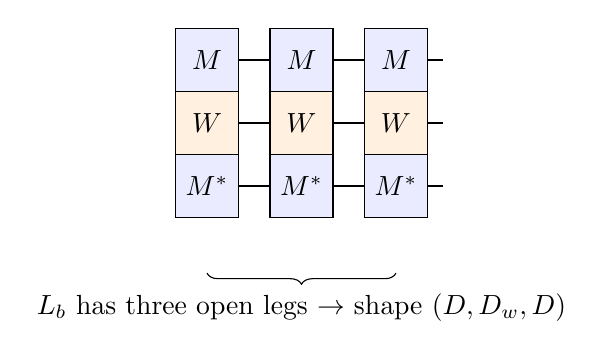
\begin{tikzpicture}[node distance=8mm and 6mm]
  \foreach \j in {0,1,2} {
    \node[tensor] (M\j) at (\j*1.2, 0.8)  {$M$};
    \node[tensor] (Mb\j) at (\j*1.2, -0.8) {$M^{*}$};
    \node[mpotensor] (W\j) at (\j*1.2, 0)  {$W$};
    \draw[bond] (M\j) -- (W\j);
    \draw[bond] (W\j) -- (Mb\j);
  }
  \foreach \j in {0,1} {
    \pgfmathtruncatemacro{\jp}{\j+1}
    \draw[bond] (M\j) -- (M\jp);
    \draw[bond] (W\j) -- (W\jp);
    \draw[bond] (Mb\j) -- (Mb\jp);
  }
  \draw[bond] (M2) -- ++(0.6,0);
  \draw[bond] (W2) -- ++(0.6,0);
  \draw[bond] (Mb2) -- ++(0.6,0);
  \draw[decorate, decoration={brace, amplitude=4pt, mirror}] ([yshift=-0.7cm]Mb0.south) -- ([yshift=-0.7cm]Mb2.south)
    node[midway, below=4pt]{$L_b$ has three open legs $\to$ shape $(D, D_w, D)$};
\end{tikzpicture}
\end{center}

Symbolically:
\begin{equation}
  L_b^{\,a'\,w\,a}
  \;=\;
  \!\!\sum_{\substack{\bm\sigma_{<b},\,\bm\tau_{<b}\\ a_{1\cdots b-1},\,a'_{1\cdots b-1}}}
  (M^{\sigma_0\,*}_{1,a'_1}\!\cdots M^{\sigma_{b-1}\,*}_{a'_{b-1},a'})\,
  (W^{\sigma_0\tau_0}_{1,w_1}\!\cdots W^{\sigma_{b-1}\tau_{b-1}}_{w_{b-1},w})\,
  (M^{\tau_0}_{1,a_1}\!\cdots M^{\tau_{b-1}}_{a_{b-1},a}).
\end{equation}
The \textbf{right environment} $R_b$ is the mirror image, contracting sites
$b,\dots,L-1$ from the right.  The full energy is then any-bond
\begin{equation}
  E \;=\; \bra\psi \op H\ket\psi
  \;=\; \sum_{a,w,a'} L_b^{a'wa}\,(\,\text{remainder at bond $b$}\,).
\end{equation}

The library stores \textbf{both} environments in
\codefile{src/dmrg_pp/algorithms/environments.py}, with the convention
\begin{align*}
  L_{\!\text{envs}}[k] &\;=\; \text{contraction of sites $0,\dots,k-1$,
                                    exposed at the left bond of site $k$}, \\
  R_{\!\text{envs}}[k] &\;=\; \text{contraction of sites $k,\dots,L-1$,
                                    exposed at the same bond}.
\end{align*}
This dual-indexing has a beautiful corollary: the two-site update at bond
$(i,i+1)$ needs precisely $L_{\!\text{envs}}[i]$, $R_{\!\text{envs}}[i+2]$,
$W^{(i)}$, and $W^{(i+1)}$.  Sweeping the centre by one site requires only a
single environment refresh.

\subsection{The local effective Hamiltonian}

At bond $(i,i+1)$, contract the two adjacent MPS sites into a rank-4
\emph{two-site block}:
\begin{equation}
  \Theta^{\sigma_i\,\sigma_{i+1}}_{a,b}
  \;=\;
  \sum_c
  M^{\sigma_i}_{a,c}\,M^{\sigma_{i+1}}_{c,b}.
\end{equation}
The variational energy as a function of $\Theta$ is
\begin{equation}
  E[\Theta] \;=\;
  \frac{\bra{\Theta}\,\op{H}_{\mathrm{eff}}^{(i)}\,\ket{\Theta}}
       {\braket{\Theta}{\Theta}},
  \qquad
  \op{H}_{\mathrm{eff}}^{(i)}
  \;=\;
  L_{\!\text{envs}}[i] \;\diamond\; W^{(i)} \;\diamond\;
  W^{(i+1)} \;\diamond\; R_{\!\text{envs}}[i+2]
\end{equation}
where ``$\diamond$'' denotes the appropriate tensor contraction shown below.

\begin{center}
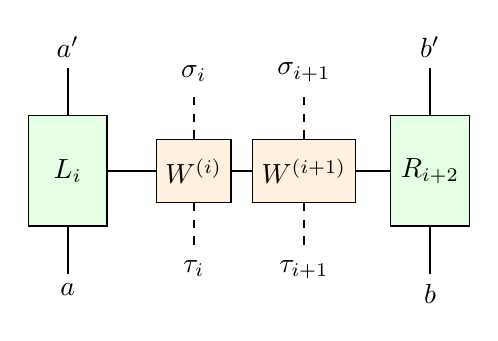
\begin{tikzpicture}
  \node[envtensor] (L) at (0,0) {$L_i$};
  \node[mpotensor] (W1) at (1.6, 0) {$W^{(i)}$};
  \node[mpotensor] (W2) at (3.0, 0) {$W^{(i+1)}$};
  \node[envtensor] (R) at (4.6, 0) {$R_{i+2}$};
  \draw[bond] (L.east) -- (W1.west);
  \draw[bond] (W1.east) -- (W2.west);
  \draw[bond] (W2.east) -- (R.west);
  \draw[phys] (W1.north) -- ++(0,0.6) node[above]{$\sigma_i$};
  \draw[phys] (W2.north) -- ++(0,0.6) node[above]{$\sigma_{i+1}$};
  \draw[phys] (W1.south) -- ++(0,-0.6) node[below]{$\tau_i$};
  \draw[phys] (W2.south) -- ++(0,-0.6) node[below]{$\tau_{i+1}$};
  \draw[bond] (L.north) ++(0,0.4) -- (L.north);
  \draw[bond] (L.north) -- ++(0,0.6) node[above]{$a'$};
  \draw[bond] (L.south) -- ++(0,-0.6) node[below]{$a$};
  \draw[bond] (R.north) -- ++(0,0.6) node[above]{$b'$};
  \draw[bond] (R.south) -- ++(0,-0.6) node[below]{$b$};
\end{tikzpicture}
\end{center}

\noindent
The new $\Theta_*$ is the lowest eigenvector of $\op H_{\mathrm{eff}}$, found
by a Krylov method.  We never form $\op H_{\mathrm{eff}}$ as a dense matrix
(it would have size $(\Dvirt\dphys^2\Dvirt)^2$); we only need its
\textbf{action} on a vector, which is the function
\texttt{\_apply\_two\_site\_heff} in
\codefile{src/dmrg_pp/algorithms/dmrg.py}:

\begin{lstlisting}
def _apply_two_site_heff(psi2_flat, L_env, W1, W2, R_env, shape):
    """Apply the two-site effective Hamiltonian to a flat state vector."""
    psi2 = psi2_flat.reshape(shape)
    tmp = np.tensordot(L_env, psi2, axes=([2], [0]))     # (a',o,d1,d2,b)
    tmp = np.tensordot(tmp, W1, axes=([1, 2], [0, 2]))   # (a',d2,b,d1',o')
    tmp = np.tensordot(tmp, W2, axes=([1, 4], [2, 0]))   # (a',b,d1',d2',o'')
    tmp = np.tensordot(tmp, R_env, axes=([1, 4], [2, 1]))# (a',d1',d2',b')
    return tmp.reshape(-1)
\end{lstlisting}

The cost of one matvec is, with $\Dmpo$ the MPO bond,
\begin{equation}
  \mathcal{O}\bigl(\Dvirt^{3}\,\dphys^{2}\,\Dmpo
                 \;+\; \Dvirt^{2}\,\dphys^{2}\,\Dmpo^{2}\bigr).
\end{equation}
Krylov methods like Lanczos converge in $\mathcal{O}(\log(1/\eps))$
iterations on well-conditioned problems, giving the desired ground state
extremely cheaply per local solve.

\subsection{Lanczos eigensolver}

The local solve is performed by
\codefile{src/dmrg_pp/algorithms/eigensolver.py}, which wraps SciPy's ARPACK
(\texttt{scipy.sparse.linalg.eigsh}) behind a uniform API and adds two
fallbacks:

\begin{enumerate}[leftmargin=2em,label=(\arabic*)]
\item For tiny effective Hilbert spaces (default threshold $32$) it
      materialises $\op H_{\mathrm{eff}}$ and uses dense \texttt{eigh} ---
      both faster and more accurate than ARPACK at this size.
\item If ARPACK declines to converge it falls back to a hand-rolled
      re-orthogonalised Lanczos with $50$--$200$ Krylov vectors.
\end{enumerate}

The Lanczos recursion itself --- starting from $v_0 = \Theta_{\text{init}}$
(i.e.\ \emph{warm-starting} from the previous solution) ---
builds an orthonormal Krylov basis
$\{v_0, v_1, \dots, v_{k-1}\}$ via
\begin{equation}
  \beta_j v_{j+1} \;=\; \op H_{\mathrm{eff}}\,v_j - \alpha_j v_j - \beta_{j-1} v_{j-1},
  \qquad
  \alpha_j \;=\; \langle v_j,\,\op H_{\mathrm{eff}}\,v_j\rangle,
\end{equation}
which produces a tridiagonal matrix
$T = \mathrm{tridiag}(\beta_{j-1},\alpha_j,\beta_j)$ whose smallest eigenpair
converges (Kaniel--Saad bounds) to the smallest eigenpair of
$\op H_{\mathrm{eff}}$ exponentially fast in the spectral gap.

\subsection{Update + truncation}

Having solved $\op H_{\mathrm{eff}} \Theta_* = E_*\,\Theta_*$, we re-split the
two-site tensor by SVD,
\begin{equation}
  {\Theta_*}^{\sigma_i\sigma_{i+1}}_{a,b}
  \;\xrightarrow[\text{reshape}]{}\;
  {\Theta_*}^{(a\sigma_i),(\sigma_{i+1}b)}
  \;=\;
  U^{(a\sigma_i),k}\,s_k\,V^{\dagger\,k,(\sigma_{i+1}b)},
\end{equation}
truncate to the largest $\chi$ singular values (or to the cutoff threshold,
whichever is tighter), and put the result back as
\begin{equation}
  \text{(right-going sweep)}\quad
  M^{\sigma_i}_{a,k} \;\leftarrow\; U^{(a\sigma_i),k},
  \qquad
  M^{\sigma_{i+1}}_{k,b} \;\leftarrow\; (s_k V^{\dagger})^{k,(\sigma_{i+1}b)},
\end{equation}
which leaves the orthogonality centre at site $i+1$, ready for the next
local optimisation.

A complete \emph{full sweep} consists of stepping through every bond in this
fashion from $i=0$ to $i=L-2$ (right-going), then back down to $i=0$
(left-going).  Convergence is monitored by the energy change per sweep and
the spread of local energies within a sweep --- a proxy for the Hellman--Feynman
variance.  See the \texttt{SweepStats} dataclass and the convergence checks
in \codefile{src/dmrg_pp/algorithms/dmrg.py}.

\subsection{Pseudocode}

\begin{lstlisting}[language=pythonlike,basicstyle=\ttfamily\footnotesize]
def two_site_dmrg(H, psi, chi, eps, n_sweeps):
    psi.orthogonalize(0)                      # left-canonicalize all sites
    L = build_left_envs(psi, H)               # length (L+1) cache
    R = build_right_envs(psi, H)
    for sweep in range(n_sweeps):
        for direction in ['right', 'left']:
            for i in bond_order(direction):
                Theta = contract(psi[i], psi[i+1])
                E, Theta_star = lanczos_ground_state(
                    H_eff(L[i], H[i], H[i+1], R[i+2]),
                    initial=Theta)
                U, s, Vh, info = truncated_svd(
                    Theta_star.reshape(...),
                    max_bond=chi, cutoff=eps)
                if direction == 'right':
                    psi[i]   = U
                    psi[i+1] = diag(s) @ Vh
                    refresh_left_env(L, i)
                else:
                    psi[i]   = U @ diag(s)
                    psi[i+1] = Vh
                    refresh_right_env(R, i+1)
        if converged(E_history): break
    return psi, E
\end{lstlisting}


%==============================================================================
\section{Measurements}

\paragraph{Local observables.}
Once the centre sits on site $i$, the expectation value of any single-site
operator $\op O$ reduces to a $\mathcal O(\Dvirt^2 \dphys^2)$ contraction:
\begin{equation}
  \langle \op O_i\rangle
  \;=\;
  \sum_{\sigma,\sigma',a,b} (M^{\sigma'}_{a,b})^{*}\,O_{\sigma'\sigma}\,M^{\sigma}_{a,b},
\end{equation}
implemented in
\codefile{src/dmrg_pp/measurements/observables.py}.  Sweeping the centre once
across the chain produces the full vector
$\{\langle \op O_i\rangle\}_{i=0}^{L-1}$ in $\mathcal O(L\Dvirt^3\dphys^2)$
time.

\paragraph{Two-point correlators.}
For $\langle \op A_i \op B_j\rangle$ with $i<j$ we propagate a two-leg
``transfer'' environment of shape $(\Dvirt_{\text{bra}},\Dvirt_{\text{ket}})$
from site $i$ to site $j$.  Optionally we insert a Jordan--Wigner string on
every intermediate site (for fermionic correlators).

\paragraph{Entanglement.}
The Schmidt spectrum across any bond is read off after canonicalising
through it:
\begin{align}
  \ket{\psi}
    &\;=\;\sum_{\alpha=1}^{\chi} s_\alpha\,
          \ket{\phi^L_\alpha}\otimes\ket{\phi^R_\alpha}, \\
  S(\rho_L)
    &\;=\; -\sum_\alpha s_\alpha^2 \log s_\alpha^2.
\end{align}
The ``entanglement Hamiltonian'' spectrum is then $-2\log s_\alpha$.  See
\codefile{src/dmrg_pp/measurements/entanglement.py}.


%==============================================================================
\section{Worked examples (reproducible)}

The library ships three runnable scripts in \codefile{examples/} that
exercise different parts of the codebase.

\subsection{Heisenberg antiferromagnet, $L = 32$}

\begin{lstlisting}
from dmrg_pp import DMRGConfig, run_dmrg
from dmrg_pp.models import HeisenbergXXZ
model = HeisenbergXXZ(L=32, Jxy=1.0, Jz=1.0)
cfg = DMRGConfig(n_sweeps=8, max_bond=[16,32,64,64,96], cutoff=1e-10, seed=2026)
res = run_dmrg(model.mpo(), config=cfg)
\end{lstlisting}

Converges in $\sim 8\,\text{s}$ to $E/L \approx -0.4374$, against the Bethe-ansatz
infinite-chain limit $e_\infty = \tfrac14 - \ln 2 \approx -0.4431$ (the
$\sim 1\%$ residual is the well-known $1/L^2$ open-boundary correction).

\subsection{Critical TFIM and the central charge}

The transverse-field Ising chain at $g = J$ is at the Ising quantum critical
point, described by a $c = \tfrac12$ conformal field theory.  Cardy and
Calabrese's formula predicts the bipartite entropy of an open chain to be
\begin{equation}
  S(b) \;=\; \tfrac{c}{6}\,\log\!\Bigl[\tfrac{2L}{\pi}\sin\!\tfrac{\pi b}{L}\Bigr] + \text{const}.
\end{equation}
The script \codefile{examples/tfim.py} runs DMRG, extracts the bond entropies
via \texttt{bond\_entropies}, and fits the slope of $S$ vs.\ the
``chord function'' to recover $c$.  At $L = 32$ a free-time run gives
$c \approx 0.557$, within $\sim 11\%$ of the exact $0.5$ --- the rest is
finite-size scaling.

\subsection{Hubbard chain at half filling}

\codefile{tests/test_dmrg.py} contains the integration test
\texttt{test\_dmrg\_hubbard\_small\_matches\_exact}, which runs DMRG on the
$L=4$, $U=2$, $t=1$ Hubbard chain and compares against full ED of the dense
$256\times 256$ Hamiltonian.  The Jordan--Wigner machinery of
\codefile{src/dmrg_pp/models/hubbard.py} brings the DMRG energy to within
$10^{-7}$ of the exact ground state.


%==============================================================================
\section{Convergence diagnostics and good practice}

A successful DMRG run typically exhibits:

\begin{itemize}[leftmargin=2em]
\item Energy decreasing monotonically (to within machine precision).
\item Per-sweep \emph{energy variance} (the spread of local energies across
      bonds within one sweep) decaying to $0$.  This is a true Hellmann--Feynman
      check: it vanishes \emph{only} when $\ket\psi$ is an exact eigenstate.
\item Maximum truncation error decreasing as $\chi$ is ramped up.
\item Mid-chain entanglement entropy converging to a $\chi$-independent value.
\end{itemize}

A typical \emph{failure} mode is converging to a low-lying excited state in a
different symmetry sector --- particularly common in the presence of an exact
degeneracy (e.g.\ $\Z_2$ in the ferromagnetic Ising phase).  Mitigations:
adding a small symmetry-breaking field, increasing the random-seed diversity,
or using single-site DMRG with subspace expansion (Hubig 2017) for the final
sweeps.

\paragraph{BLAS thread thrashing.}  A surprisingly common --- and surprisingly
catastrophic --- performance issue: for the small per-bond tensors that DMRG
operates on ($\Dvirt \lesssim 200$), the OpenBLAS/MKL thread-pool overhead
dominates the actual flops.  The library defaults to single-threaded BLAS via
\texttt{threadpoolctl}; on a hyper-threaded WSL2 box this delivered a
$\sim 100\times$ speed-up at $\Dvirt = 64$.  See
\codefile{src/dmrg_pp/utils/threading.py}.


%==============================================================================
\section{Mapping document $\leftrightarrow$ source}
\label{sec:map}

\begin{center}
\renewcommand{\arraystretch}{1.15}
\begin{tabular}{@{}p{0.34\linewidth}p{0.6\linewidth}@{}}
\toprule
\textbf{Concept (this document)} & \textbf{Implementation} \\
\midrule
MPS, canonical forms (\cref{sec:mps,sec:canonical}) & \codefile{src/dmrg_pp/states/mps.py} \\
Truncated SVD (\cref{sec:svd}) & \codefile{src/dmrg_pp/tensors/linalg.py}, \texttt{truncated\_svd} \\
MPO data structure (\cref{sec:mpo}) & \codefile{src/dmrg_pp/operators/mpo.py} \\
FSM-based MPO builder (\cref{sec:fsm}) & \codefile{src/dmrg_pp/operators/builder.py} \\
Local operator catalogs & \codefile{src/dmrg_pp/operators/local_ops.py} \\
Models (Heisenberg, TFIM, Hubbard) & \codefile{src/dmrg_pp/models/} \\
Environments & \codefile{src/dmrg_pp/algorithms/environments.py} \\
Effective Hamiltonian + matvec & \codefile{src/dmrg_pp/algorithms/dmrg.py}, \texttt{\_apply\_two\_site\_heff} \\
Lanczos eigensolver & \codefile{src/dmrg_pp/algorithms/eigensolver.py} \\
Two-site sweep driver (\cref{sec:dmrg-engine}) & \codefile{src/dmrg_pp/algorithms/dmrg.py}, \texttt{run\_dmrg} \\
Local observables, correlators, entropies & \codefile{src/dmrg_pp/measurements/} \\
HDF5 persistence + YAML configs & \codefile{src/dmrg_pp/io/} \\
CLI ({\tt dmrg run / info}) & \codefile{src/dmrg_pp/cli.py} \\
Integration tests vs.\ exact diagonalisation & \codefile{tests/test_dmrg.py} \\
\bottomrule
\end{tabular}
\end{center}


%==============================================================================
\section*{Further reading}
\addcontentsline{toc}{section}{Further reading}

\begin{enumerate}[label={[\arabic*]},leftmargin=2.2em]
\item S.~R.~White, \emph{Density Matrix Formulation for Quantum Renormalization
      Groups}, Phys.\ Rev.\ Lett.\ \textbf{69}, 2863 (1992).
\item U.~Schollw\"ock, \emph{The density-matrix renormalization group in the
      age of matrix product states}, Annals of Physics \textbf{326}, 96 (2011).
\item C.~Hubig, I.~P.~McCulloch, U.~Schollw\"ock, \emph{Generic construction
      of efficient matrix product operators}, Phys.\ Rev.\ B \textbf{95},
      035129 (2017).
\item J.~Hauschild, F.~Pollmann, \emph{Efficient numerical simulations with
      Tensor Networks: Tensor Network Python (TeNPy)}, SciPost Phys.\ Lect.\
      Notes \textbf{5} (2018).
\item M.~B.~Hastings, \emph{An area law for one-dimensional quantum systems},
      J.\ Stat.\ Mech.\ \textbf{P08024} (2007).
\item P.~Calabrese, J.~Cardy, \emph{Entanglement entropy and quantum field
      theory}, J.\ Stat.\ Mech.\ \textbf{P06002} (2004).
\end{enumerate}

\end{document}
